\subsection{Graphit}
Die Graphitschicht konnte magnetisch auf der Probenhalterung angebracht werden. Die Vorbereitungen f�r die Graphitmessung dauerten nicht lange, da nach wenigen Versuchen eine funktionsf�hige Pt-Ir-Spitze angefertigt werden konnte. F�r die Anfertigung der Pt-Ir-Spitze standen Isopropanol, Reinigungst�cher, eine Pinzette und eine Zange zu halten des Drahtes. Um den Pt-Ir-Draht anzuspitzen, stand uns ein Seitenschneider zur Verf�gung, mit dem der Draht angeschnitten wurde, sodass durch darauffolgendes kr�ftiges Ziehen eine (idealerweise) einatomige Spitze erzeugt werden konnte.
Nachdem eine passende Pt-Ir-Spitze hergestellt werden konnte, wurde mit dem RTM ein Bereich von 600nm im "`Topographie"'-Modus (CC) abgerastert.
Die dazu ben�tigten Einstellungen konnten mit dem Programm f�r das RTM eingestellt werden und sind in Tabelle \ref{tab:para_topo_graph} dargestellt.
\begin{table}[H]
\centering
\caption{Parameter zur Topographiemessung (CC-Mode)}
\begin{tabular}{c|c}
Variable & Wert\\
\hline Set point & \SI{1}{nA}\\
P-gain & 1000\\
I-gain & 1700\\
Tip-voltage & \SI{50}{mV}\\
\end{tabular}
\label{tab:para_topo_graph}
\end{table}
Die Topographiemessung �ber \SI{600}{nm} ist in Abbildung \ref{fig:topo_graph_600nm} dargestellt.
\begin{figure}[H]
\centering
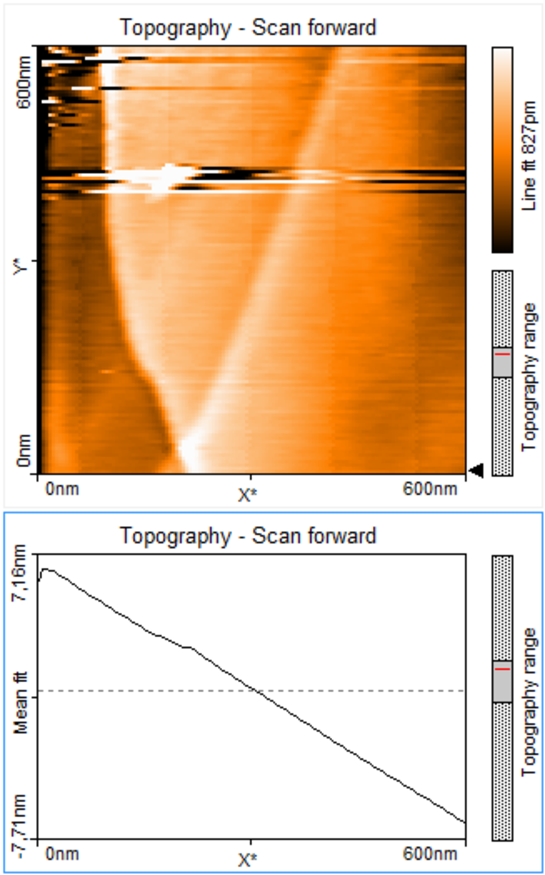
\includegraphics[scale = 0.75,clip = true, trim = 0cm 6.2cm 0cm 0cm]{ausschnitt_600}
\caption{ \SI{600}{nm} Bild im Topographie/CC-Modus }
\label{fig:topo_graph_600nm}
\end{figure}
\subsubsection{Rauheit}
Die Rauheit der Graphitschicht konnte mit der Software f�r das RTM bestimmt werden, nachdem die Graphitschicht im CC-Modus mit der Spitze des RTM abgerastert wurde. Die Verkippung wurde bestimmt und korrigiert. Das Fenster Topography-Scan ist f�r die Messung nicht wichtig, da es die Oberfl�chenbeschaffenheit ausschlie�lich auf H�he des schwarzen Pfeils angibt. In Abbildung \ref{fig:lin_rau_graph} ist die Messung zur Bestimmung der mittleren Linienrauheit dargestellt.
\begin{figure}[H]
\centering
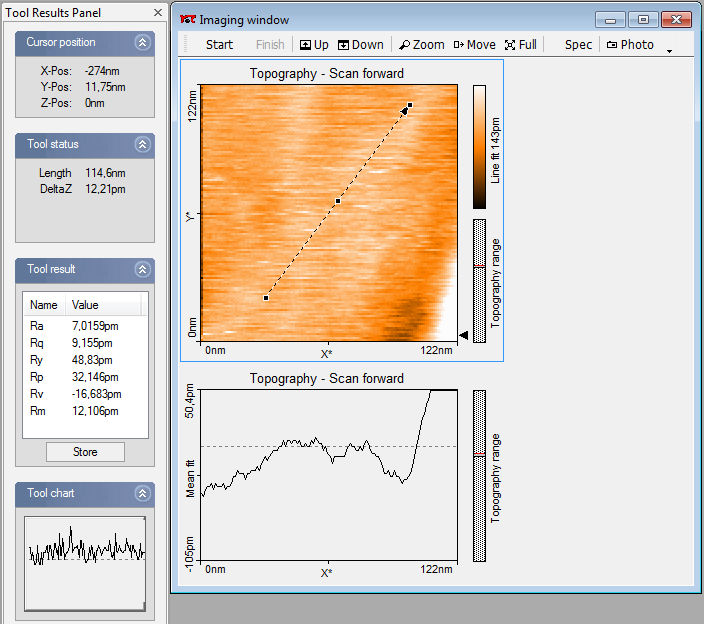
\includegraphics[scale = 0.75]{snipping_122_linienrauheit}
\caption{ Mittlere Linienrauheit von Graphit ($R_a = \SI{7,0159}{pm}$ und $R_q = \SI{9,155}{pm}$) }
\label{fig:lin_rau_graph}
\end{figure}
Ebenso wurde die mittlere Fl�chenrauheit der Graphitprobe bestimmt, welche in Abbildung \ref{fig:flae_rau_graph} dargestellt ist.
\begin{figure}[H]
\centering
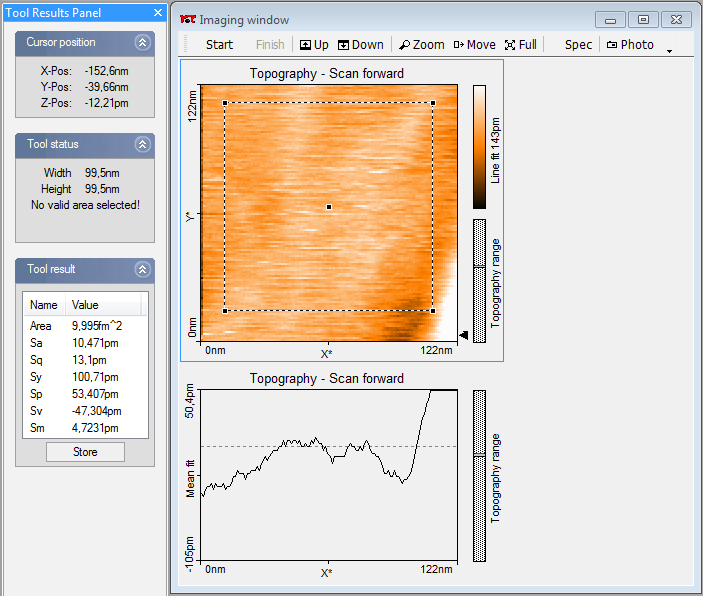
\includegraphics[scale = 0.75]{snipping_122_flaechenrauheit}
\caption{ Mittlere Fl�chenrauheit von Graphit ($S_a = \SI{10,471}{pm}$ und $S_q = \SI{13,1}{pm}$) }
\label{fig:flae_rau_graph}
\end{figure}
\subsubsection{Gitterstruktur und Elektronendichteverteilung}
\subsubsection{Mittlerer Atomabstand}